\section{Acelerômetro}		
	Um acelerômetro é um componente eletrônico que mede as forças exercidas num determinado objeto.  Essas forças podem ser de 
	dois tipos: estáticas ou dinâmicas, sendo estática a força da aceleração gravitacional (constante), e dinâmicas 
	causadas pelo movimento ou vibração provocados no acelerômetro \cite[p. 20]{LISBOA}.

	
	\subsection{Funcionamento}
	O princípio básico de um acelerômetro é a ação de aceleração de uma massa para produzir força, conforme descrito na 
	segunda lei de Newton (vide Equação \ref{eq:segunda}):

	\begin{equation}
		F = m \times a,
		\label{eq:segunda}
	\end{equation}
	onde $F$ é a força em Newtons [N], $m$ a massa em quilos [kg] e $a$ aceleração em $m/{s^2}$. Portanto, é necessário a utilização de uma massa nos acelerômetros, chamada massa inercial para medir a aceleração \cite[p. 271]{INSTRUME}. O acelerômetro pode ser modelado matematicamente como mostra na Figura \ref{fig:modeloAcc}.\\	 

		\begin{figure}[H]
		\vspace{4mm}
		\centering
		\caption{Modelo de um acelerômetro que consiste em uma massa sísmica, um elemento mola e um elemento amortecimento}		
		\label{fig:modeloAcc}	
		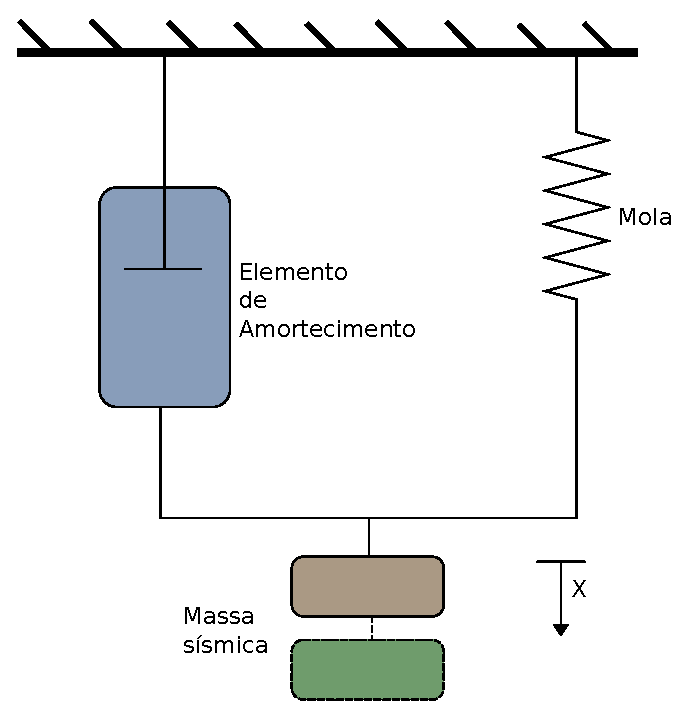
\includegraphics[scale=0.7]{imagens/massamola.eps}
		\caption*{Fonte: \citeonline[p. 271]{INSTRUME}.}
		\end{figure}
	
	Conforme a Figura \ref{fig:modeloAcc}, uma força pode ser aplicada a massa de acordo com a segunda lei de Newton, e o esquema pode ser modelado conforme \cite{INSTRUME}:
	\begin{equation}
		\frac{x(s)}{a(s)} = \frac{1}{ 	s^2 + \frac{b}{m} + s\frac{K}{m}},
		\label{eq:laplace}
	\end{equation}
	em que $s$ representa o operador de Laplace, $x$ o deslocamento da massa de sua posição de repouso, $a$ a aceleração a ser mensurada, $b$ o coeficiente de amortecimento, $m$ a massa destinada ao movimento e $K$ a constante da mola.
	
	Os acelerômetros são encontrados em diversos tamanhos e tecnologias, entre eles os piezoelétricos, piezorresistivos e capacitivos. Para reduzir o tamanho do dispositivo,são aplicadas técnicas da área de microeletrônica, resultando em um dispositivo classificado como sistema
	microeletromecânico ou MEMS (Micro-Electro-Mechanical System). \cite{INSTRUME}.

	\subsection{Eixos de rotação}
Conforme \citeonline{NASA} uma aeronave em pleno voo irá rotacionar em torno do seu centro de gravidade, que é o ponto de onde se localiza a massa média da aeronave. É possível definir um sistema de coordenadas tridimensional baseado no centro de gravidade onde, cada eixo é perpendicular a outros dois eixos. Logo é possível definir a orientação pela quantidade de rotação das partes da aeronaves em relação aos eixos principais \cite{NASA}. Na Figura \ref{fig:rotations} observa-se uma aeronave com o sistema de coordenadas baseados nas rotações.
        
        \begin{figure}[H]
        	\vspace{4mm}
            \centering
            \caption{Aeronave com o sistema de coordenadas baseado nas rotações}
            \label{fig:rotations}
            \includegraphics[scale=0.5]{imagens/rotations.png}

            \caption*{Fonte: \citeonline{NASA}.}

        \end{figure}
        
        O eixo nomeado de \textit{Yaw} ($\psi$) é definido como perpendicular as asas do avião, tem origem no centro de gravidade e é direcionado para baixo (via Figura \ref{fig:rotations}). O eixo \textit{Pitch} ($\theta$) é perpendicular ao eixo \textit{Yaw} e paralelo as asas da aeonave, com origem no centro de gravidade e tem a direção das asas.
        O eixo \textit{Roll} ($\phi$) é perpendicular aos outros eixos, com origem no centro de gravidade e é direcionado ao nariz da aeronave.
        
        Observando estes eixos e definindo no sensor inercial, para distinguir as letras que possuem movimento será necessário somente o eixo de rotação \textit{Roll}, como pode ser observado na Figura \ref{fig:mpu_eixos}.
        
        \begin{figure}[H]
        	\vspace{4mm}
            \centering
            \caption{Sensor inercial com o eixo de \textit{Roll} definido}
            \label{fig:mpu_eixos}
            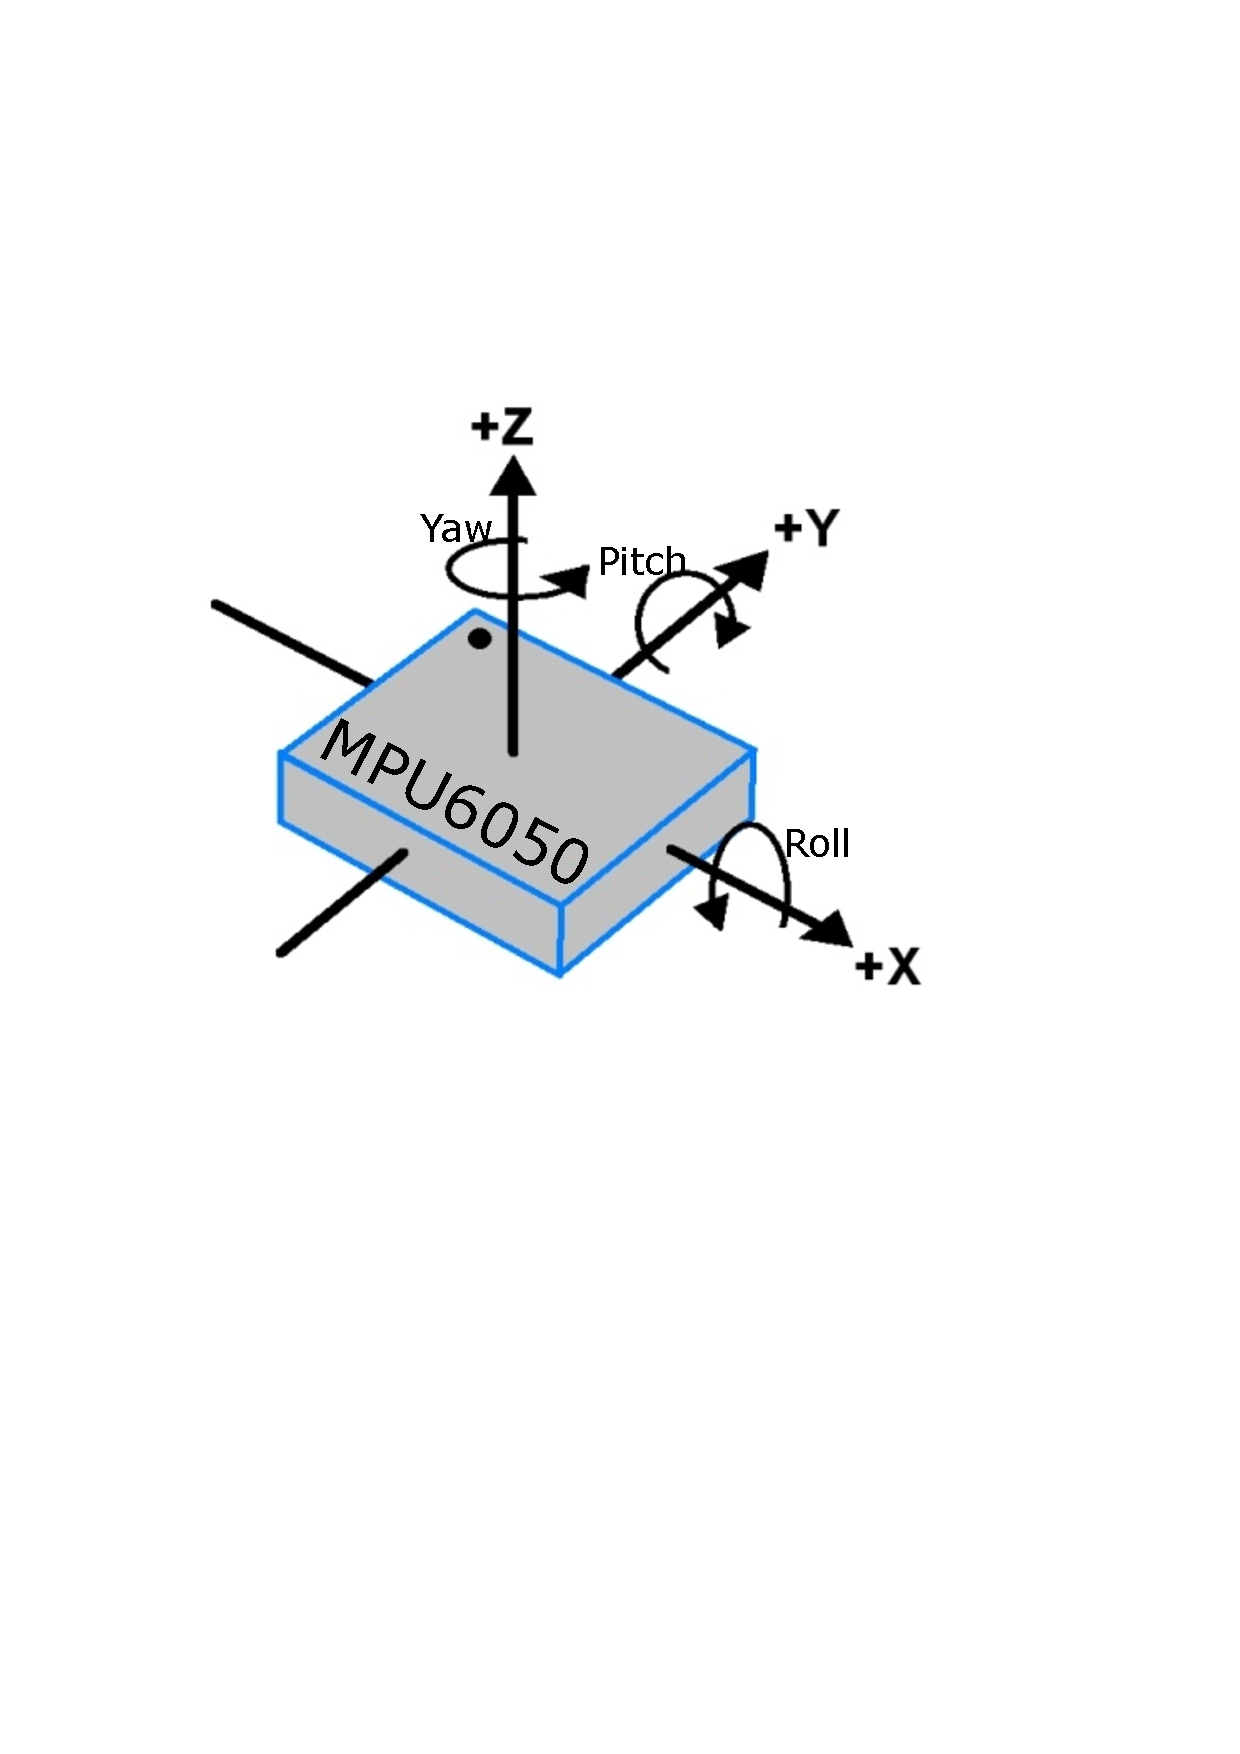
\includegraphics[scale=0.3, trim={4cm 14cm 6cm 7cm}, clip]{imagens/ypr2.png}
            \caption*{Fonte: Adaptado de \citeonline{eixos}.}
        \end{figure}
        
        
        De acordo com \citeonline{nxp:acell}, o acelerômetro dos celulares é utilizado para definir a orientação da tela utilizando o sistema de coordenadas tridimensionais. Logo é possível obter os eixos \textit{Pitch} e \textit{Roll} a partir dos valores dos 3 eixos do acelerômetro.
        
        Assumindo que o acelerômetro é orientado no campo gravitacional da terra $g$ e passa por aceleração linear $a_r$ medido no \textit{frame} de referência da terra $r$, terá uma saída dada por \cite{nxp:acell}:
        \begin{equation}
            G_p = 
            \begin{pmatrix}
                G_{px} \\
                G_{py} \\
                G_{pz}
            \end{pmatrix}    
             = R (g - a_r),
            \label{eq:ROLL1}
        \end{equation}
        onde $R$ é a matriz de rotação que descreve a orientação do acelerômetro com relação as coordenadas da terra.
        
        
        Supõe-se que o acelerômetro não tem aceleração linear ( necessário assumir isso para resolver a Equação \ref{eq:ROLL1} para a matriz de rotação $R$), quando houver presença de aceleração linear será adicionado um erro na estimação da orientação. Também assume-se que a orientação inicial do acelerômetro é plana com o campo gravitacional da terra e alinhado com o eixo $z$. Considerando isso, a saída $G_p$ do acelerômetro é demonstrada por \cite{nxp:acell} (medido em $g$):	
        
        \begin{equation}
            G_p = 
            \begin{pmatrix}
                G_{px} \\
                G_{py} \\
                G_{pz}
            \end{pmatrix}    
             = Rg = R.
             \begin{pmatrix}
                0 \\
                0 \\
                1
             \end{pmatrix}
            \label{eq:ROLL2}
            ,
        \end{equation}
        
    Para determinar os ângulos \textit{Yaw, Pitch} e \textit{Roll}, é necessário descrever as componentes da matriz de rotação $R$. As matrizes de rotação \textit{Yaw}($R_z(\psi)$), \textit{Pitch}($R_y(\theta)$) e \textit{Roll} ($R_x(\phi)$) transformam o vetor $G_p$ sobre uma rotação do sistema de coordenadas da Figura \ref{fig:mpu_eixos}
    para ângulos de \textit{Roll} ($\phi$), \textit{Pitch} ($\theta$), e \textit{Yaw} ($\psi$). Essas matrizes são expressas como \cite{nxp:acell}:
    \begin{equation}
        R_x(\phi) = 
        \begin{pmatrix}
            1 & 0 & 0\\
            0 & cos \phi & sin \phi\\
            0 & -sin \phi & cos \phi
        \end{pmatrix}
        \label{eq:ROLL3}
        ,
    \end{equation}
    
    \begin{equation}
        R_y(\theta) = 
        \begin{pmatrix}
            cos \theta & 0 & -sin \theta \\
            0 & 1 & 1\\
            sin \theta & 0 & cos \theta
        \end{pmatrix}
        \label{eq:ROLL4}
        ,
    \end{equation}
    ,
    \begin{equation}
        R_z(\psi) = 
        \begin{pmatrix}
            cos \psi & sin \psi & 0 \\
            -sin \psi & cos \psi & 0 \\
            0 & 0 & 1
        \end{pmatrix}
        \label{eq:ROLL5}
        .
    \end{equation}
    
    Existem seis possibilidades para ordenar essas três matrizes de rotação. Em princípio, todas são igualmente válidas \cite{nxp:acell}. Considerando isso e inicialmente o valor de $1g$ no eixo $z$, resulta em  \cite{nxp:acell}:
    
    \begin{equation}
        R_{xyz}.
        \begin{pmatrix}
        0 \\ 0 \\ 1
        \end{pmatrix}
        = R_x(\phi) R_y(\theta) R_z(\psi).
        \begin{pmatrix}
            0 \\ 0 \\ 1
        \end{pmatrix}
        \label{eq:ROLL6}
        .
    \end{equation}
    
    Fazendo a substituição e a multiplicação das matrizes das Equações \ref{eq:ROLL3}, \ref{eq:ROLL4}, e \ref{eq:ROLL5} na Equação \ref{eq:ROLL6} demonstra-se que  \cite{nxp:acell}:
    
    \begin{equation}
        \begin{pmatrix}
            cos \theta cos \psi & cos \theta sin \psi & -sin \theta \\
            
            cos \psi sin \theta sin \phi - cos \phi sin \psi & 
            cos\phi cos\psi + sin \theta sin \phi sin \psi &
            cos \theta sin \phi \\
            
            cos \phi cos\psi sin \theta  + sin\phi sin\psi &
            cos \phi sin \theta sin \psi - cos \psi sin \phi &
            cos \theta cos\phi 
            
        \end{pmatrix}
        .
        \begin{pmatrix}
            0 \\ 0 \\ 1
        \end{pmatrix}
        \label{eq:ROLL7}
        ,
    \end{equation}
    efetuando a multiplicação resulta na matriz:
    
    \begin{equation}
    = 
        \begin{pmatrix}
        -sin \theta \\ cos\theta sin \phi \\ cos\theta cos \phi
        \end{pmatrix}
        \label{eq:ROLL8}
        .
    \end{equation}
    
    Reescrevendo \ref{eq:ROLL8} com base no vetor $G_p$ resulta em:

    \begin{equation}
        \frac{G_p}{|| G_p ||}
        = 
        \begin{pmatrix}
            -sin \theta \\ cos\theta sin \phi \\ cos\theta cos \phi
        \end{pmatrix}
        \Rightarrow
        \frac{1}{\sqrt{G_{px}^2 + G_{py}^2 + G_{pz}^2}}
        \begin{pmatrix} 
            G_{px} \\ G_{py} \\ G_{pz} 
        \end{pmatrix}
        =
        \begin{pmatrix}
            -sin \theta \\ cos\theta sin \phi \\ cos\theta cos \phi
        \end{pmatrix}
        \label{eq:ROLL9}
        ,
    \end{equation}
    
    
    Resolvendo \ref{eq:ROLL9} para o eixo necessário para este trabalho, que é o \textit{Roll}, tem-se:
    \begin{equation}
        tan_{xyz} \phi =  \frac{G_{py}}{G_{pz}}
        .
        \label{eq:ROLL10}
    \end{equation}
    
    Utilizando os valores de $G_{py} = 0,082198$ e $G_{pz} = -0,887432$, a resolução de \ref{eq:ROLL10} pode ser tanto $-5.29$ ou $174.71$, uma vez que os valores de \textit{Roll} variam de -180º a 180. Para solucionar este problema se utiliza da função atan2, que automaticamente retorna o ângulo em radianos no quadrante correto baseado no sinal dos dois argumentos \cite{nxp:acell}. Finalmente, chega-se a expressão para calcular o \textit{Roll} do acelerômetro:

    \begin{equation}
        \phi_{xyz} = atan2(G_{py}, G_{pz}).
        \label{eq:ROLL11}
    \end{equation}
